\subsection{Indledende designovervejelser}\label{sec:designdatabase}

Til projektet er der udviklet en database som står for at gemme alle brugerdata, herunder brugere, brugernes pools samt alle sensordata der foretages på disse pools.

Den endelige database er udviklet med Entity Frameworket, med en \textit{Model First} tilgang. Dette er valgt efter mange overvejelser og flere forsøg med forskellige udviklingsmetoder. Dette er beskrevet i detaljer i projekt dokumentationen i afnsittet om \todo{reference til dokumentationen}. I de nedenstående afsnit beskrives designet og implementeringen af både databasen og projektets data-access lag. Beskrivelserne tager udgangspunkt i de to primære user stories, som der også refereres til i resten af denne rapport. Data-access laget er som helhed omfattende af skulle beskrive. Derfor findes der yderligere information om det resterende funktionalitet og design i projektets dokumentation \todo{reference til doku}.

Databasen og data-access laget er udviklet sideløbende, og har gennemgået 3 primære udviklingsfaser. Første fase med User, derefter Pool og til sidst Data. Dette afspejles ved at der i projektet er arbejdet i iterationer, hvor der blev udviklet et funktionelt produkt for hver iteration. De mange iterationer kan da groft opdeles i disse 3 faser.

Da databasen er udviklet med \textit{Object Relational Mapperen}, Entity Framework er det lettere at arbejde med rå data, ved at give mulighed for at behandle dem som data objekter.

Data access laget er udviklet specifikt til Smartpool databasen, og er designet med henblik på usability og robustness. Denne software komponent er testet grundigt, og let at bruge for klienter.
De primære klasser og interfaces i data-access laget er følgende:

\begin{itemize}
	\item \textbf{SmartpoolDB som implementerer ISmartpoolDB.}\\
	Eksponerer et interface for klienten, \gls{windserver}.
	\item \textbf{UserAccess som implementerer IUserAccess.}\\
	Står for al database adgang og database forespørgsler i forhold til systemets brugere samt brugerinformation.
	\item \textbf{PoolAccess som implementerer IPoolAccess.}\\
	Som det ovenstående står denne klasse for al database adgang og database forespørgsler i forhold til systemets pools.
	\item DataAccess som implementerer IDataAccess.\\
	Klassen data-access er på samme måde bindeleddet til al sensor data der foretages på pools.
\end{itemize}

De fulde klassediagram for data-access laget findes i projektdokumentationens Appendix\todo{reference til dokumentation}.

De data entiteter der ses på figur~\ref{fig:databaseERD_final_uml}, findes også som C\# klasser. Det er dem der udgør database-objekterne. Som det ses på figuren, har entiteten \textit{Data} en Timestamp property, samt associationer til alle sensor-data typerne. Sensor-data typerne holder selve måleværdierne. Når der laves en forespørgsel i databasen på måledata, bruges de enkelte sensor entiteters fremmednøgle, \textit{DataId} til at finde frem til deres egentlige Timestamp.

\subsection{Udvalgte User Stories}
Med udgangspunkt i de to følgende User Stories, beskrives database designet og data-acces laget. 

\begin{itemize}
	\item \textit{"Som bruger vil jeg kunne oprette mig i systemet for at få adgang til systemet"}
	\item \textit{"Som bruger vil jeg kune se de seneste sensorværdier for at kunne få et overblik over poolens tilstand"}
\end{itemize}

\subsection{User story - Oprettelse af en bruger i systemet}

Ved at tage udgangspunkt i projektets domæneanalyse, blev det gjort klart hvilke attributter, en Bruger/User af systemet skulle have. Disse attributter er vist på figur~\ref{fig:database_model_1}.

\begin{figure}[h]
\centering
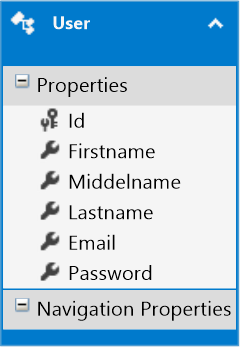
\includegraphics[width=0.2\linewidth]{figs/database/database_model_1.png}
\caption{User entiteten}
\label{fig:database_model_1}
\end{figure}


Ud fra denne entitet laves et SQL script som kan køres mod databasen. Tabellen som vises på figur~\ref{fig:usertable} er da oprettet i databasen gennem Entity Frameworket.

\begin{figure}[h]
\centering
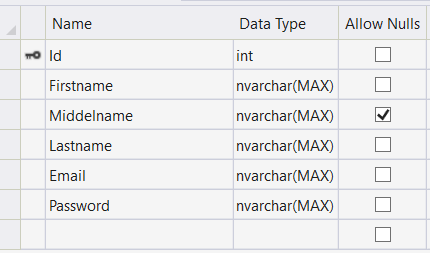
\includegraphics[width=0.5\linewidth]{figs/database/usertable}
\caption{User entitens tabel i databasen}
\label{fig:usertable}
\end{figure}


Med en funktionel database er det nu oplagt at begynde på designet af data-access laget. Der ønskes herudover funktionalitet til at tage brugere ud af databasen. I forbindelse med udarbejdelsen af disse backend funktonaliter blev \textit{Test Driven Development} brugt, hvor der blev identificeret testcases og testscenarier. Denne måde at arbejde på har også sat sit præg på data-access lagets test coverage procent, som set på figur~\ref{fig:coverage}.

\begin{figure}[h]
\centering
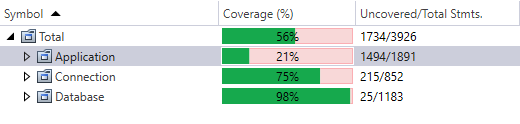
\includegraphics[width=0.75\linewidth]{figs/database/coverage.png}
\caption{Test coverage for Smartpool systemet}
\label{fig:coverage}
\end{figure}

Som testene blev skrevet, blev tilsvarende business-logic og funktionalitet implementeret.
Det har hele tiden været tanken at data-access laget skulle være nemt at bruge hos klienten, \gls{windserver}. Derfor er løsningen designet med et interface, ISmartpoolDB, som kan ses på figur~\ref{fig:classISmartpoolDB}.

\begin{figure}[h]
\centering
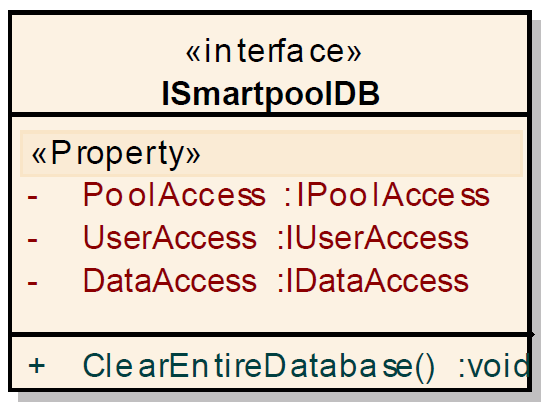
\includegraphics[width=0.3\linewidth]{figs/database/classISmartpoolDB}
\caption{Interfacet ISmartpoolDB}
\label{fig:classISmartpoolDB}
\end{figure}

På denne måde er systemet åbent for udvidelse, da der let kan tilføjes nye Access klasser. På samme måde er designet depandancy inverted.

\begin{figure}[h]
	\centering
	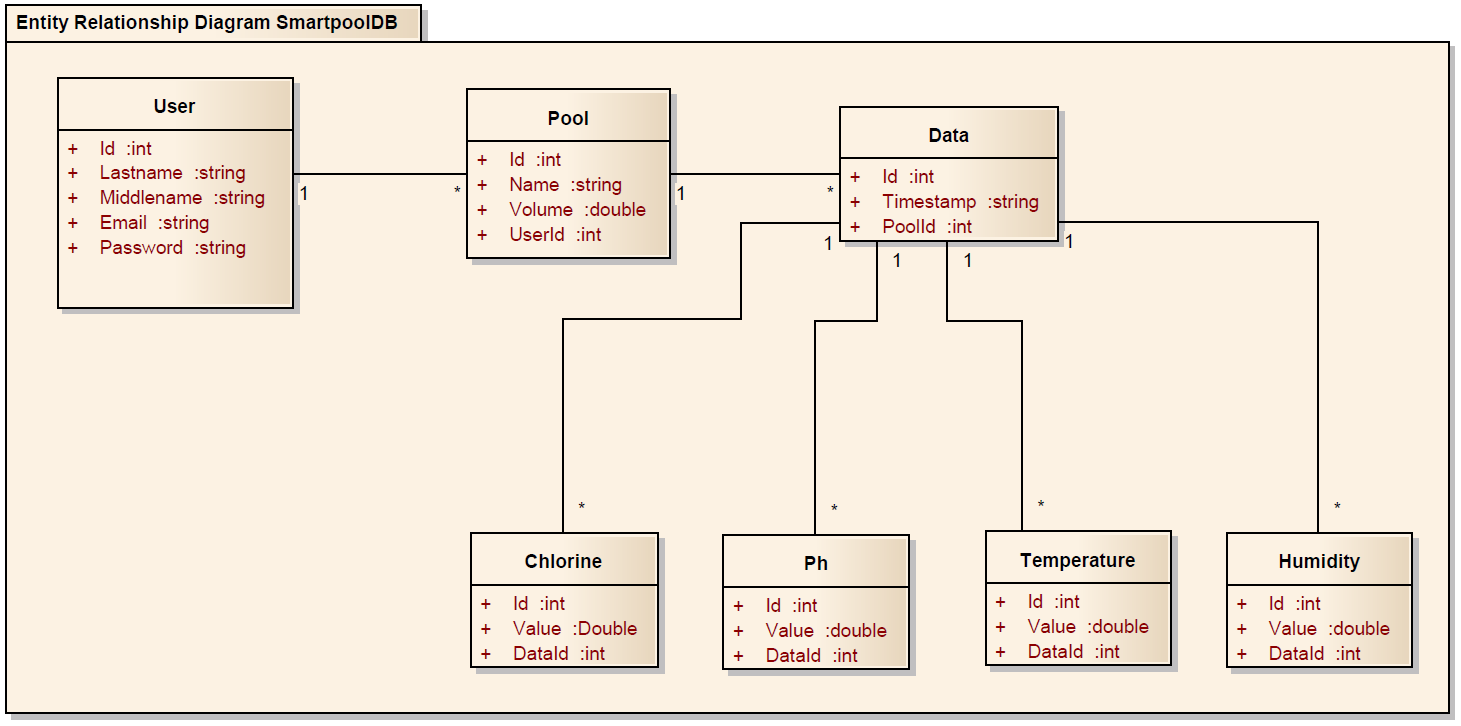
\includegraphics[width=\linewidth]{figs/design/databaseERD_final_uml}
	\caption{Endeligt ER diagram, UML notation}
	\label{fig:databaseERD_final_uml}
\end{figure}

En klient kan kalde sig ind i alt data-access lagets funktionalitet gennem ISmartpoolDB interfacet. I projektets dokumentation \todo{indsæt reference her} beskrives det hvorledes data-access laget bruges på \gls{windserver}.

\subsection{User story - Se sensor værdier}

Eftersom funktionalitet til oprettelse af Brugere/Users og Pools blev lavet, var  det tid til at gå i gang med sensordata ting.

Dette var 3 fase, og vi havde derfor en fuldt fungerende User og Pool. Måden sensordata persisteres på i databasen skiller sig en smule ud fra måden hvor fx en USer eller en pool gøres. \todo{indsæt ER diagram for data og dtatyper}. Som det kan ses på figur XXXX indeholder databasen 4 typer af sensor målinger, samt en Data entitet. Is tedet for at hver enkel sensortype entitet indeholder et timestamp, har vi valgt at ligge timestampet på Dataentiteten. Dett gøres for at det samme timestamp ikke skal ligge på flere data - undgå redundant data.  Samtidig hvis man gerne vil have ex luftfugtighed i samme tidsrum som klor level, er det vigtigt at målingernes timestamp er den samme.

Der er lavet en dataAccess klasse til at lave data wueries og skrivninger til databasen. Se klassediagra \todo{indsæt her}

Igen brugtes test driven development til dette, hvor koden blev skrevet til testene.  \todo{indæt mere test bragging}.

Der er til dataaccess lavet it interface som initialiseret af SmartpoolDB.

Måden hvorpå der trækkes data ud af databasen er ved hjælp af LINQ ueries. \todo{skriv lidt om LINQ qureis og hvordan man bruger dem}. Brugen heraf er skrevet i detaljer idokumenttionen.

Her på XXXX vises hvordan DALS getter metoder bruges af en klient.\ todo{indsæt kodeudsnit fra windserver}